\documentclass[UTF8, noindent]{ctexart}
\zihao{-5}
\setlength{\marginparsep}{0pt}
\setlength{\marginparwidth}{0pt}
\addtolength{\textwidth}{20pt}

\usepackage{graphicx}

\usepackage[bookmarks=true,unicode, linkbordercolor={1 1 1}]{hyperref}

\usepackage{listings}

\renewcommand{\lstlistingname}{{\footnotesize\bfseries code}}
\newcommand{\coderef}[1]{\lstlistingname\,\ref{#1}}

\lstset{
    basicstyle={\ttfamily\small}
    , frame=tb
    , escapeinside=``
    % , captionpos=b
}

\pagestyle{empty}

\renewcommand{\labelitemi}{-}



\title{两个经典面试题}
\author{taylor jiang}


%%%%%%%%%%%%%%%%%%%%%%%%%%%%%%%%%%%%%%%%%%%%%%%%%%%%%%%%%%%%%
\begin{document}

\maketitle

\tableofcontents

\section{问题描述}
{
\renewcommand{\labelenumi}{\bfseries\sffamily 问题\,\arabic{enumi}:}

\begin{enumerate}

\item 看下面代码:

\begin{lstlisting}
var a = 0, b = 0;
function A( a ) {
    A = function ( b ) {
        alert( a + b++ );
    };
    alert( a++ );
}
A( 1 );
A( 2 );
\end{lstlisting}

分析代码的执行结果.


\item 看下面代码:

\begin{lstlisting}
var a = { num: 2 };
var b = a;
a.num = a = { num: 4 };
console.log( a.num );
console.log( b.num );
\end{lstlisting}

分析代码的执行结果.


\end{enumerate}
}

%%%%%%%%%%%%%%%%%%%%%%%%%%%%%%%%%%%%%%%%%%%%%%%%%%%%%%%%%%%%

\section{第一题解释}

这一题的考点在:

\begin{itemize}
\item 词法作用域与变量搜索原则.
\item 函数是\,JavaScript\,中的特殊的类型, 与普通的类型数据使用方法一样.
\item 函数限定作用域, 函数的形参亦是函数内的声明.
\item 若函数内部数据可被访问, 则函数内存不会被释放.
\item 自增与自减运算符.
\end{itemize}


\subsection{分析执行步骤}

\begin{enumerate}

\item 首先, 代码进行预解析. 在\,js\,引擎中记录下三个成员, 分别是\,\lstinline|a|, \lstinline|b|, 
      和\,\lstinline|A|. 预解析不会处理函数, 也不会运行代码.
\item 然后代码就变成了如下样子:

\begin{lstlisting}
a = 0, b = 0;
A( 1 );
A( 2 );
\end{lstlisting}

\item 预解析之后, 代码开始运行. 首先执行赋值运算. 
      将数字\,\lstinline|0|\,分别存储到\emph{全局变量}\,\lstinline|a|\,和\,\lstinline|b|\,中.
\item 然后第一次调用函数\,\lstinline|A|, 传入参数\,\lstinline|1|.
\item 在函数内的执行步骤为:

    \begin{enumerate}
    \item 首先进行函数内的预解析. 由于函数内没有显式声明\footnote{var\,定义变量, 或独立的函数声明}, 
          因此该步骤容易被人忽略. 实际上函数的参数就是在函数内部的第一个声明, 
          即在函数内部有局部的变量\,\lstinline|a|\,存在. 并且其值在函数调用时赋值为\,\lstinline|1|.
    \item 然后依次执行函数内部的代码. 
    \item 首先对\,\lstinline|A|\,进行赋值. 根据变量的搜索规则\footnote{在访问变量时, 如果当前函数内没有变量的声明, 则到上一级作用域查找.}, 
          \lstinline|A|\,就是函数的引用, 因此给\,\lstinline|A|\,赋值后, 
          相当于修改\emph{全局函数}\,\lstinline|A|\,的指向, \lstinline|A|\,指向匿名函数:
{\begin{lstlisting}[caption={\footnotesize 匿名函数}, label=fn]
function ( b ) {
    alert( a + b++ );
}
\end{lstlisting}}

          然后调用\,\lstinline|alert|\,函数, 打印\,\lstinline|a++|\,的结果.
    \item 然而根据后置运算符\,\lstinline|++|\,的特征, 表达式\,\lstinline|a++|\,的取值为原值, 
          取值后\,\lstinline|a|\,的值累加一次. 即表达式的值为\,\lstinline|1|, 
          而后\,\lstinline|a|\,的值为\,\lstinline|2|.
    \item 所以\,\lstinline|alert|\,此时打印出来的结果为\,\lstinline|1|.
    \item 由于全局变量\,\lstinline|A|\,引用了匿名函数(\,如\,\coderef{fn}), 所以当前函数执行结束后, 不会立即释放函数内存. 
          即保存了变量\,\lstinline|a|\,不被释放(\,构成闭包结构\,). 函数执行结束.
    \end{enumerate}

\item 然后回到代码的外层执行环境. 继续执行代码. 然后第二次调用函数\,\lstinline|A|, 并传入参数\,\lstinline|2|.

\item 函数的内部执行为:

    \begin{enumerate}
    \item 由于第一次执行函数\,\lstinline|A|\,的时候, 已重新让\,\lstinline|A|\,指向了匿名函数\,\coderef{fn}. 因此调用函数\,\lstinline|A|,
          实际上是在调用匿名函数.
    \item 因此首先进行函数内预解析, 发现有局部变量\,\lstinline|b|, 并且取值为\,\lstinline|2|.
    \item 然后调用\,\lstinline|alert|\,函数, 打印表达式\,\lstinline|a + b++|\,的结果.
    \item 根据后置自增运算符的运算规则, 表达式中\,\lstinline|b++|\,的值为\,\lstinline|2|, 取值后\,\lstinline|b|\,的值为\,\lstinline|3|.
    \item 而根据闭包中保存的变量\,\lstinline|a|\,的值为\,\lstinline|2|\,可知, 表达式\,\lstinline|a + b++|\,的值为\,\lstinline|4|.
    \item 因此\,\lstinline|alert|\,打印出\,\lstinline|4|. 函数执行结束.
    \end{enumerate}

\item 最后代码执行结束.

\end{enumerate}



\section{第二题解释}

这一题的考点在\footnote{该案例涉及到词法分析, 相对来说优点复杂. 如果理解不是很好, 可以先记下来.}:

\begin{itemize}
\item 引用类型的变量存储的只是一个地址.
\item js\,代码从左往右, 从上往下解释运行.
\item 代码的执行是按照运算符的结合顺序进行, 但是这个结合顺序往往被人们经验所想当然.
\item js\,对象具有动态特性\footnote{只要对象存在, 点赋值即可为对象创建新的成员}.
\item 词法分析, 连续赋值运算符构成一个栈内存结构.
\end{itemize}


\subsection{代码分析}

\begin{enumerate}

\item 首先代码预解析, 得到两个全局变量\,\lstinline|a|\,和\,\lstinline|b|;
\item 然后执行代码, 根据代码的运行, 第一行代码执行完, 其内存逻辑相当于:

{\centering\noindent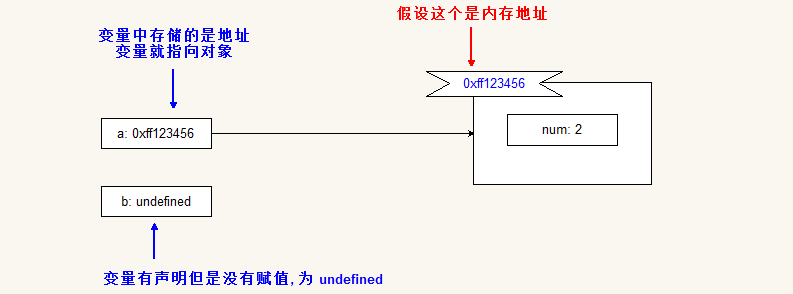
\includegraphics[width=0.9\textwidth]{imgs/2018-01-16_155948.png}}

\item 然后执行第二段代码, 将变量\,\lstinline|a|\,中存储的\emph{地址}赋值给变量\,\lstinline|b|. 其内存逻辑为:

{\centering\noindent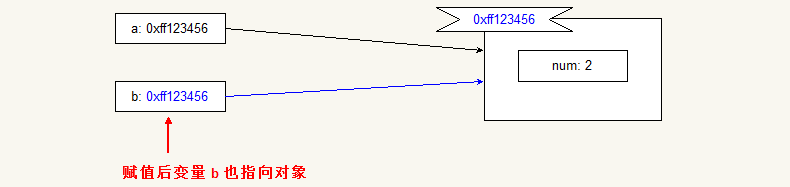
\includegraphics[width=0.9\textwidth]{imgs/2018-01-16_160904.png}}

\item 接着最复杂的一句话: \lstinline|a.num = a = { num: 4 }|. 在这段代码中, 代码的执行时从左往右的, 
      但是赋值运算符是从右往左结合的. 也就是说, 如果有代码:
    
\begin{lstlisting}
console.log( 1 + 2 + 3 * 4 ); // 15
\end{lstlisting}

      在这段代码中, 代码执行的顺序是什么呢? 可以先思考一下.

      按照成年人的一般计算规律, 我们都知道先算乘除, 再算加减. 因此, 很容易将代码的计算变成先计算\,\lstinline|3 * 4|,
      得到结果后, 再计算\,\lstinline|1 + 2 + 12|. 最终计算的结果是\,\lstinline|15|. 
      答案没有任何问题. 这是因为加法满足交换律, 运算\,$1+2+3*4$\,与运算\,$3*4+1+2$\,等价.
      但是这与计算机的运算是不一样的. 因为计算机的运算是\emph{从左往右, 从上到下}的计算.

      那么在计算机中, 上面的代码运行是, 先计算\,\lstinline|1 + 2|, 然后求得\,\lstinline|3|.
      在读入代码\,\lstinline|+ 3 * 4|, 发现后续运算是乘法, 因此无法在刚刚得到的结果上计算加法.
      因此将刚刚得到的结果存储起来(\,入栈\,), 先计算\,\lstinline|3 * 4|\,的结果, 得到\,\lstinline|12|.
      再将存储的数据取出(\,出栈\,), 再把这两个数相加, 即\,\lstinline|3 + 12|, 最后求得结果.
      其计算顺序逻辑图为:
    
{\noindent\centering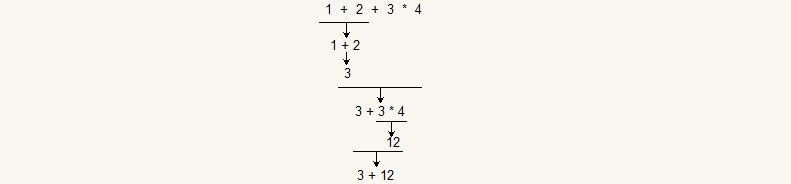
\includegraphics[width=0.9\textwidth]{imgs/2018-01-16_165539.png}}

\item 回头过来看我们的代码: 
    \begin{enumerate}
    \item \lstinline|a.num = a = { num: 4 }|, 代码从左往右读取, 首先看到\,\lstinline|a.num =|, 
          但是它现在不参与计算, 因此会将其存储起来(\,入栈\,), 最后再计算. 
    \item 然后读入\,\lstinline|a = |, 依旧不参与运算. 因此入栈.
    \item 此时需要注意的是两次入栈, 入的是什么. 第一次入栈, 是通过\,\lstinline|a|\,取得\,\lstinline|num|.
          而\,\lstinline|a|\,本身不存储数据, 存储的是一个地址, 因此\,\lstinline|a.num|\,是找到了对象中的一个属性.
          因此第一次入栈的是对象中的属性\,\lstinline|num|.

          而第二次入栈的是变量\,\lstinline|a|. 其内存的逻辑图可以看成:

{\noindent\centering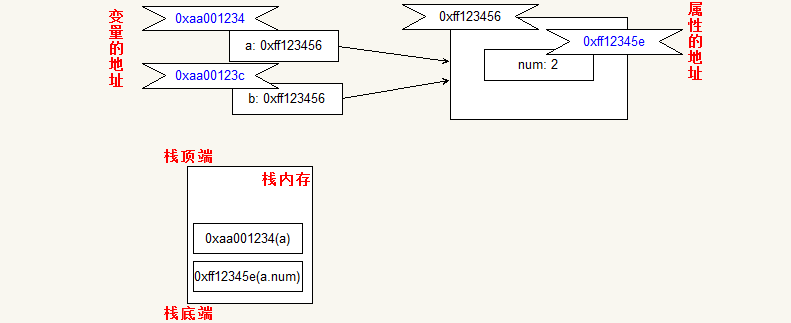
\includegraphics[width=0.86\textwidth]{imgs/2018-01-16_170427.png}}

    \item 然后得到一个新的对象\,\lstinline|{ num: 4 }|. 进行第一次赋值, 将其地址赋值给变量\,\lstinline|a|. 
          内存逻辑图为:
    
{\noindent\centering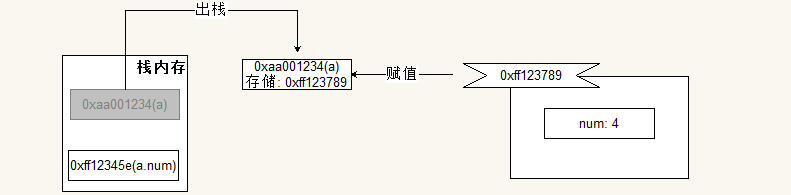
\includegraphics[width=0.86\textwidth]{imgs/2018-01-16_171209.png}}

          然后内存中变量的引用关系就编程了:
          
{\noindent\centering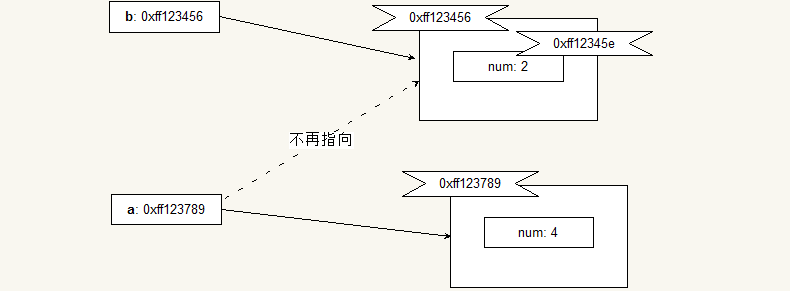
\includegraphics[width=0.86\textwidth]{imgs/2018-01-16_171500.png}}

    \item 赋值表达式的值为等号右边的值, 即在完成该赋值后, 再取出栈底的\,\lstinline|a.num|, 
          但是这仅仅是形式表达式, 因为\,\lstinline|a|\,的执行已经变量. 但是这没关系, 
          因此实际上出栈的是原来对象的\,\lstinline|num|\,属性. 即逻辑图所示:

{\noindent\centering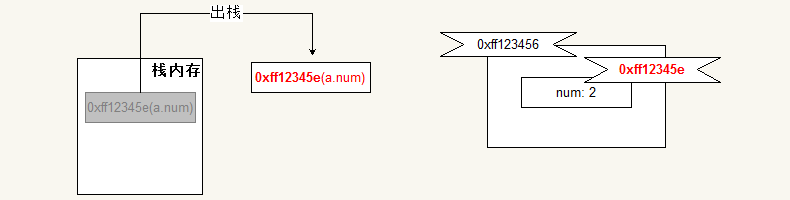
\includegraphics[width=0.86\textwidth]{imgs/2018-01-16_171913.png}}

          然后赋值给它, 内存中数据的指向关系又发生了变化, 图为:
        
{\noindent\centering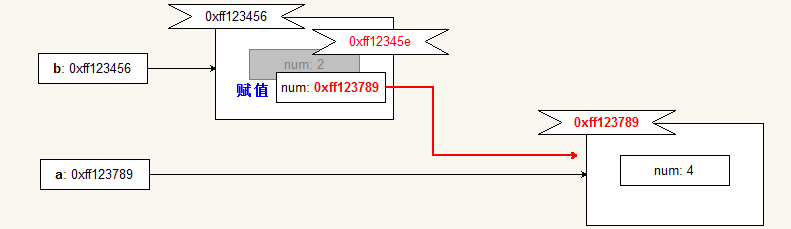
\includegraphics[width=0.86\textwidth]{imgs/2018-01-16_172407.png}}

    \item 该赋值运算语句结束后, 根据逻辑图, 对象\,\lstinline|a|\,已经重新指向; 
          而变量\,\lstinline|b|\,依旧执行原来的对象. 但是原来对象的\,\lstinline|num|\,属性也发生了变化,
          它不再存储数字, 而是指向了新的对象.

    \end{enumerate}

\item 最后打印两个变量对应的\,\lstinline|num|\,值, 根据逻辑图很显然. 为了验证这个逻辑, 可以修改代码:

\begin{lstlisting}
var a = { num: 2, text: '`旧`' };
var b = a;
a.num = a = { num: 4, text: '`新`' };
console.log( a.num );
console.log( b.num );
\end{lstlisting}

      根据前面的分析, 也可以绘制出它的内存指向逻辑图:
      
{\noindent\centering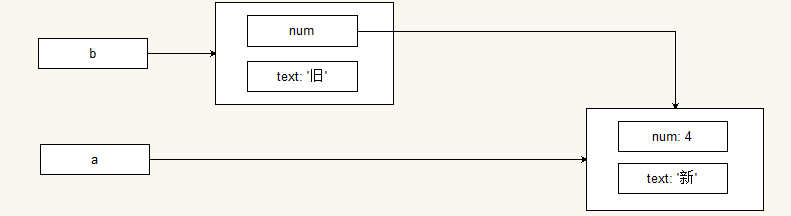
\includegraphics[width=0.9\textwidth]{imgs/2018-01-16_172956.png}}

      将代码运行后, 在调试工具下验证有:

{\noindent\centering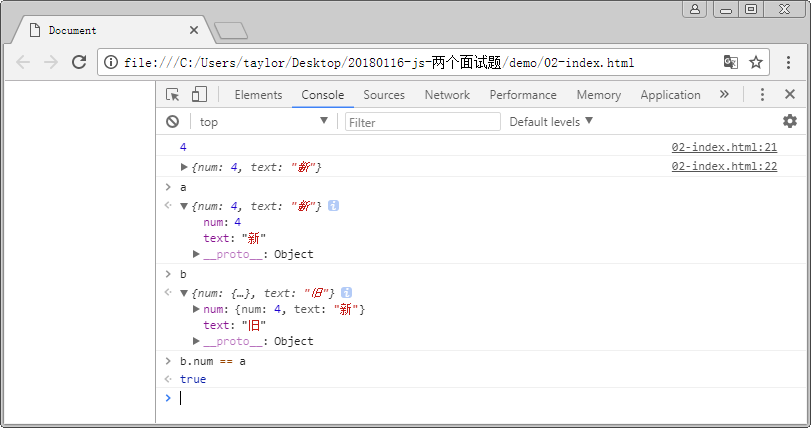
\includegraphics[width=0.9\textwidth]{imgs/2018-01-16_173153.png}}

      显然与绘制的逻辑结构一致.

\end{enumerate}





\end{document}